% !TEX root = ../FundationsDataScience.tex

\chapter{Convex Optimization}
\label{chap-conv-duality}

The main references for this chapter are~\cite{chambolle2010introduction,chambolle2016introduction,boyd2004convex}, see also~\cite{parikh2014proximal,boyd2011distributed,beck2014introduction}. 


We consider a general convex optimization problem
\eql{\label{eq-general-pbm} % eq-min-smooth-uncons
	\umin{x \in \Hh} f(x)
}
where $\Hh=\RR^N$ is a finite dimensional Hilbertian (i.e. Euclidean) space, 
and try to devise ``cheap'' algorithms with a low computational cost per iterations. The class of algorithms considered are first order, i.e. they make use of gradient information. 


%%%%%%%%%%%%%%%%%%%%%%%%%%%%%%%%%%%%%%%%%%%%%%%%%%%%%%%%%%%%%%%%%%%%%%%%%%%%%%%%%%
%%%%%%%%%%%%%%%%%%%%%%%%%%%%%%%%%%%%%%%%%%%%%%%%%%%%%%%%%%%%%%%%%%%%%%%%%%%%%%%%%%
%%%%%%%%%%%%%%%%%%%%%%%%%%%%%%%%%%%%%%%%%%%%%%%%%%%%%%%%%%%%%%%%%%%%%%%%%%%%%%%%%%
\section{Gradient Descent Methods}
\label{sec-grad-descent}

We have already encountered the gradient descent method informally in Section~\ref{}�for the regularization of inverse problem. We now give a detailed analysis of the method.

%%%%%%%%%%%%%%%%%%%%%%%%%%%%%%%%%%%%%%%%%%%%%%%%%%%%%%%%%%%%%%%%%%%%%%%%%%%%%%%%%%
\subsection{Gradient Descent}

The optimization program~\eqref{eq-ip-tv-eps} is a example of unconstrained convex optimization of the form~\eqref{eq-general-pbm} where $f : \Hh \rightarrow \RR$ is a $\Cc^1$ function with Lipschitz gradient (so-called ``smooth'' function). Recall that the gradient $\nabla f : \Hh \mapsto \Hh$ of this functional (not to be confound with the discretized gradient $\nabla x \in \Hh$ of $f$) is defined by the following first order relation
\eq{
	f(x+r) = f(x) + \dotp{f}{r}_{\Hh} + O(\norm{r}_{\Hh}^2)
}
where we used $O(\norm{r}_{\Hh}^2)$ in place of $o(\norm{r}_{\Hh})$ (for differentiable function) because we assume here $f$ is of class $\Cc^1$ (i.e. the gradient is continuous). Section~\ref{eq-example-grad} shows typical examples of gradient computation.

For such a function, the gradient descent algorithm is defined as
\eql{\label{eq-grad-desc}
	\iit{x} \eqdef \it{x} - \tau_\ell \nabla f( \it{x} ), 
}
where the step size $\tau_\ell>0$ should be small enough to guarantee convergence, but large enough for this algorithm to be fast.

One also needs to quantify the smoothness of $f$. This is enforced by requiring that the gradient is $L$-Lipschitz, i.e.
\eql{\label{eq-lipsch-grad}\tag{$\Rr_L$}
	\foralls (x,x') \in \Hh^2, \quad
	\norm{ \nabla f(x)-\nabla f(x') } \leq L \norm{x-x'}. 
}
In order to obtain fast convergence of the iterates themselve, it is needed that the function has enough ``curvature'' (i.e. is not too flat), which corresponds to imposing that $f$ is $\mu$-strongly convex
\eql{\label{eq-strong-conv}\tag{$\Ss_\mu$}
	\foralls (x,x'), \in \Hh^2, \quad
	\dotp{\nabla f(x)-\nabla f(x')}{ x-x' } \geq \mu \norm{x-x'}^2. 
}
The following proposition express these conditions as constraints on the hessian for $\Cc^2$ functions.

\begin{prop}
Conditions~\eqref{eq-lipsch-grad} and~\eqref{eq-strong-conv} imply
\eql{\label{eq-above-below-quad}
	\foralls (x,x'), \quad
	f(x') + \dotp{\nabla f(x)}{x'-x} + \frac{\mu}{2}\norm{x-x'}^2
	\leq
	f(x) 
	\leq 
	f(x') + \dotp{\nabla f(x')}{x'-x} + \frac{L}{2}\norm{x-x'}^2.
}
If $f$ is of class $\Cc^2$, conditions~\eqref{eq-lipsch-grad} and~\eqref{eq-strong-conv} are equivalent to
\eql{\label{eq-upper-lower-bound-hess}
	\foralls x, \quad \mu \Id_{N \times N}  \preceq \partial^2 f(x) \preceq L \Id_{N \times N}
}
where $\partial^2 f(x) \in \RR^{N \times N}$ is the Hessian of $f$, and 
where $\preceq$ is the natural order on symmetric matrices, i.e.
\eq{
	A \preceq B \quad\Longleftrightarrow\quad
	\foralls x \in \Hh, \quad \dotp{A u}{u} \leq \dotp{B u}{u}.
}
\end{prop}
\begin{proof}
	We prove~\eqref{eq-above-below-quad}, using Taylor expansion with integral remain
	\eq{
		f(x') - f(x) = \int_0^1 \dotp{\nabla f(x_t)}{x'-x} \d t
		= \dotp{\nabla f(x)}{x'-x} + \int_0^1 \dotp{\nabla f(x_t)-\nabla f(x)}{x'-x} \d t		
	}
	where $x_t \eqdef f+t(x'-x)$.
	%
	Using Cauchy-Schwartz, and then the smoothness hypothesis~\eqref{eq-lipsch-grad}
	\eq{
		f(x') - f(x) \leq \dotp{\nabla f(x)}{x'-x} +  \int_0^1 L \norm{x_t-f} \norm{x'-x} \d t
		\leq \dotp{\nabla f(x)}{x'-x} +  L \norm{x'-x}^2 \int_0^1  t  \d t
	} 
	which is the desired upper-bound. Using directly~\eqref{eq-strong-conv} gives 
	\eq{
		f(x') - f(x) 
		= \dotp{\nabla f(x)}{x'-x} + \int_0^1 \dotp{\nabla f(x_t)-\nabla f(x)}{\frac{x_t-x}{t}} \d t	
		\geq \dotp{\nabla f(x)}{x'-x} + \mu \int_0^1 \frac{1}{t}\norm{x_t-x}^2  \d t
	}
	which gives the desired result since $\norm{x_t-x}^2 / t = t \norm{x'-x}^2$.
\end{proof}

The relation~\eqref{eq-above-below-quad} shows that a smooth (resp. strongly convex) functional is bellow a quadratic tangential majorant (resp. minorant). 

Condition~\eqref{eq-upper-lower-bound-hess} thus reads that the singular values of $\partial^2 f(x)$ should be contained in the interval $[\mu,L]$. The upper bound is also equivalent to $\norm{\partial^2 f(x)}_{\text{op}} \leq L$ where $\norm{\cdot}_{\text{op}}$ is the operator norm, i.e. the largest singular value. 
%
In the special case of a quadratic function $\Qq$ of the form~\eqref{eq-quad-func}, $\partial^2 f(x)=A$ is constant, so that $[\mu,L]$ can be chosen to be the range of the singular values of $A$.

The following theorem ensure the convergence of the gradient descent with a linear speed.

\begin{thm}\label{thm-gradsec-strong-conv}
	If $f$ satisfy conditions~\eqref{eq-lipsch-grad} and~\eqref{eq-strong-conv}, assuming there exists $(\tau_{\min},\tau_{\max})$ such that
	\eql{\label{eq-descent-step-cond}
		0 < \tau_{\min} \leq \tau_\ell \leq \tau_{\max} < \frac{2 \mu}{L}
	}
	then there exists $0 \leq \rho<1$ such that 
	\eql{\label{eq-global-linrate-grad}
		\norm{ \it{x}-x^\star } \leq \rho^\ell \norm{\itz{x}-x^\star}
	} 
	where $x^\star$ is the unique solution to~\eqref{eq-min-smooth-uncons}. 
\end{thm}
\begin{proof}
	Since $\nabla f(x^\star)=0$, one has
	\eq{
		\iit{x}-x^\star = (\it{x}-x^\star) - \tau_\ell ( \nabla f(\it{x})-\nabla f(x^\star) ).
	}
	Hence, using strong convexity and Lipschitz gradient
	\begin{align*}
		\norm{\iit{x}-x^\star }^2 &= \norm{ \it{x}-x^\star }^2 - 2\tau_\ell \dotp{\it{x}-x^\star}{\nabla f(\it{x})-\nabla f(x^\star)}
		+ \tau_\ell^2 \norm{\nabla f(\it{x})-\nabla f(x^\star)}^2 \\
		& \leq P(\tau_\ell) \norm{ \it{x}-x^\star }^2 
		\qwhereq
		P(\tau) = 1-2 \mu \tau + L^2 \tau^2. 
	\end{align*}
	Figure~\ref{fig-grad-desc-contract}, left,�shows visually the shape of the second order polynomial $P$, which shows that condition~\eqref{eq-descent-step-cond} on $\tau_\ell$ implies
	\eq{
		P(\tau_\ell)^{\frac{1}{2}} \leq \rho \eqdef \max( P(\tau_{\min}), P(\tau_{\max}) )^{\frac{1}{2}}< 1, 
	}
	which shows the desired result.
\end{proof}


\begin{figure}
\centering
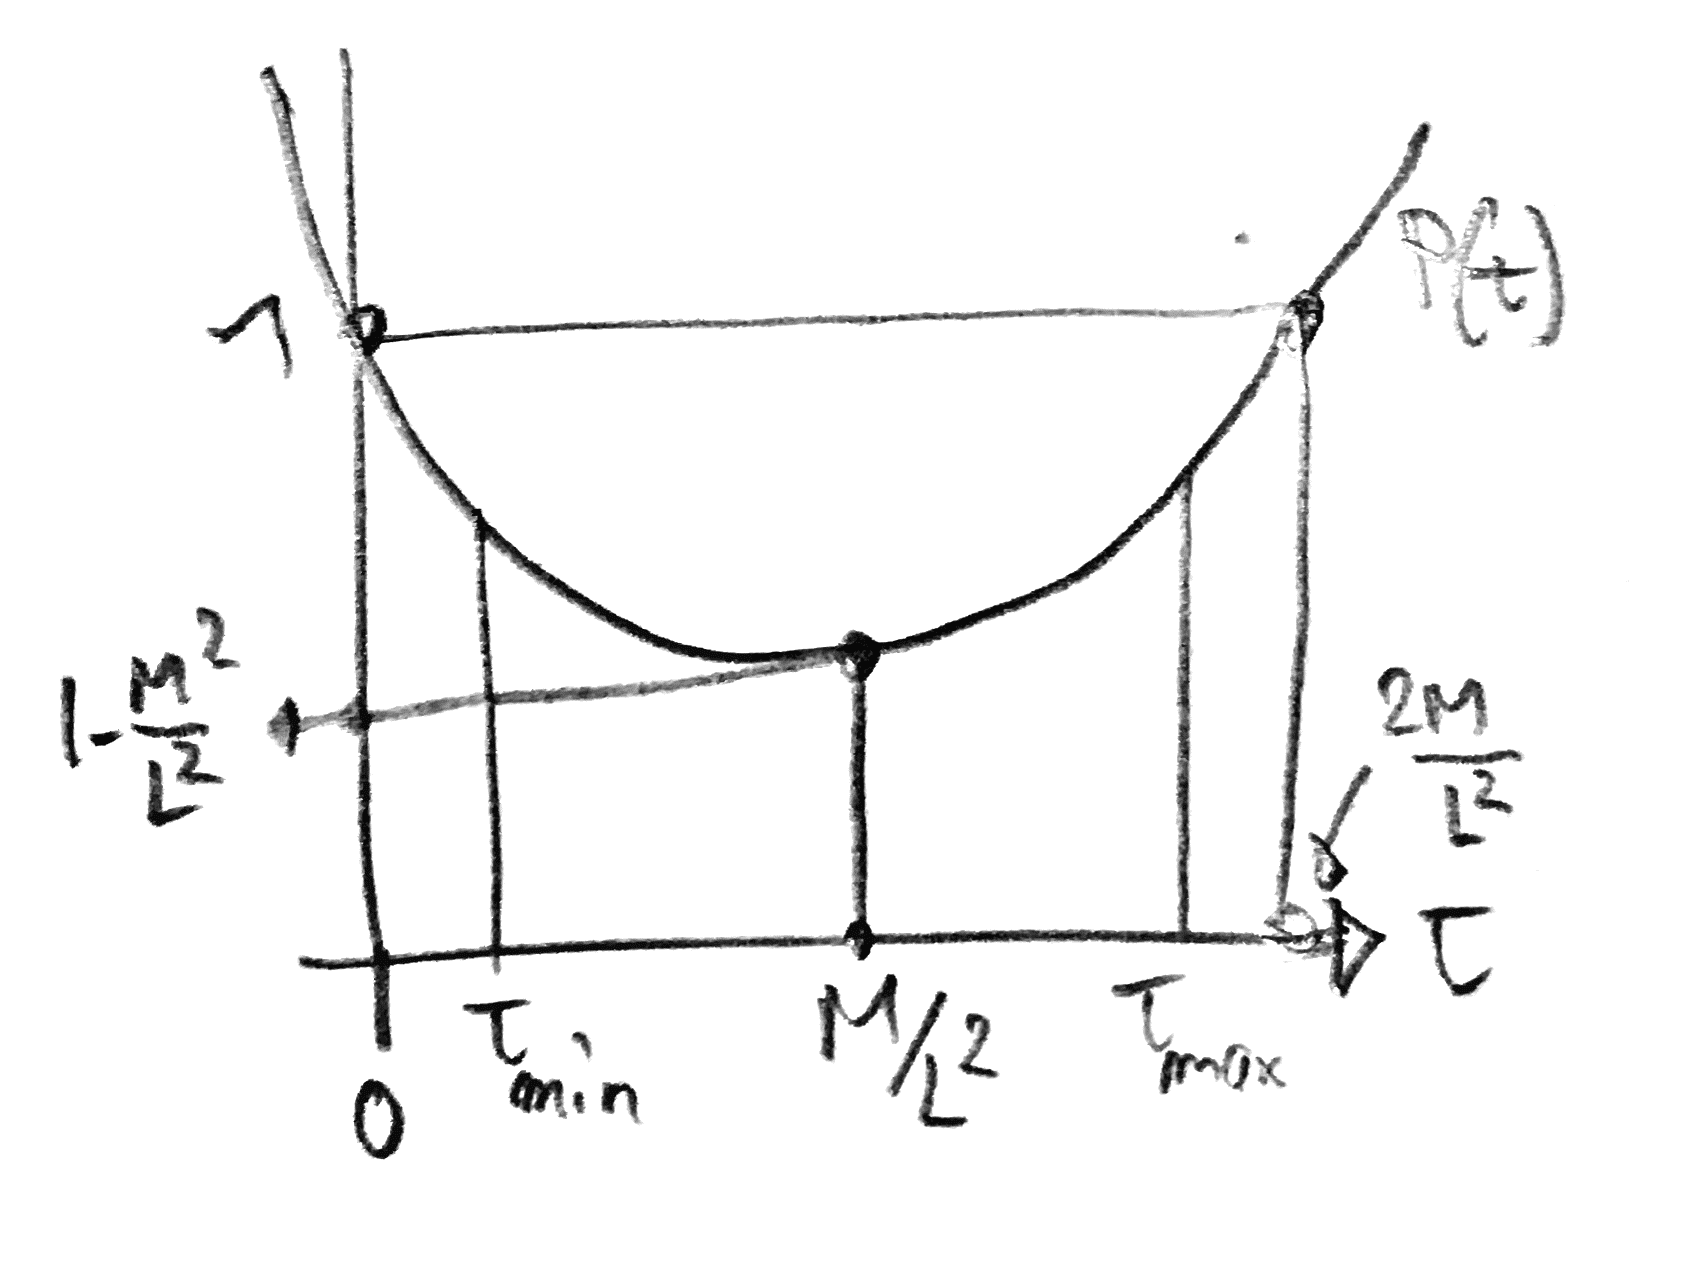
\includegraphics[width=.35\linewidth]{inverse-problems/grad-desc-general} \quad
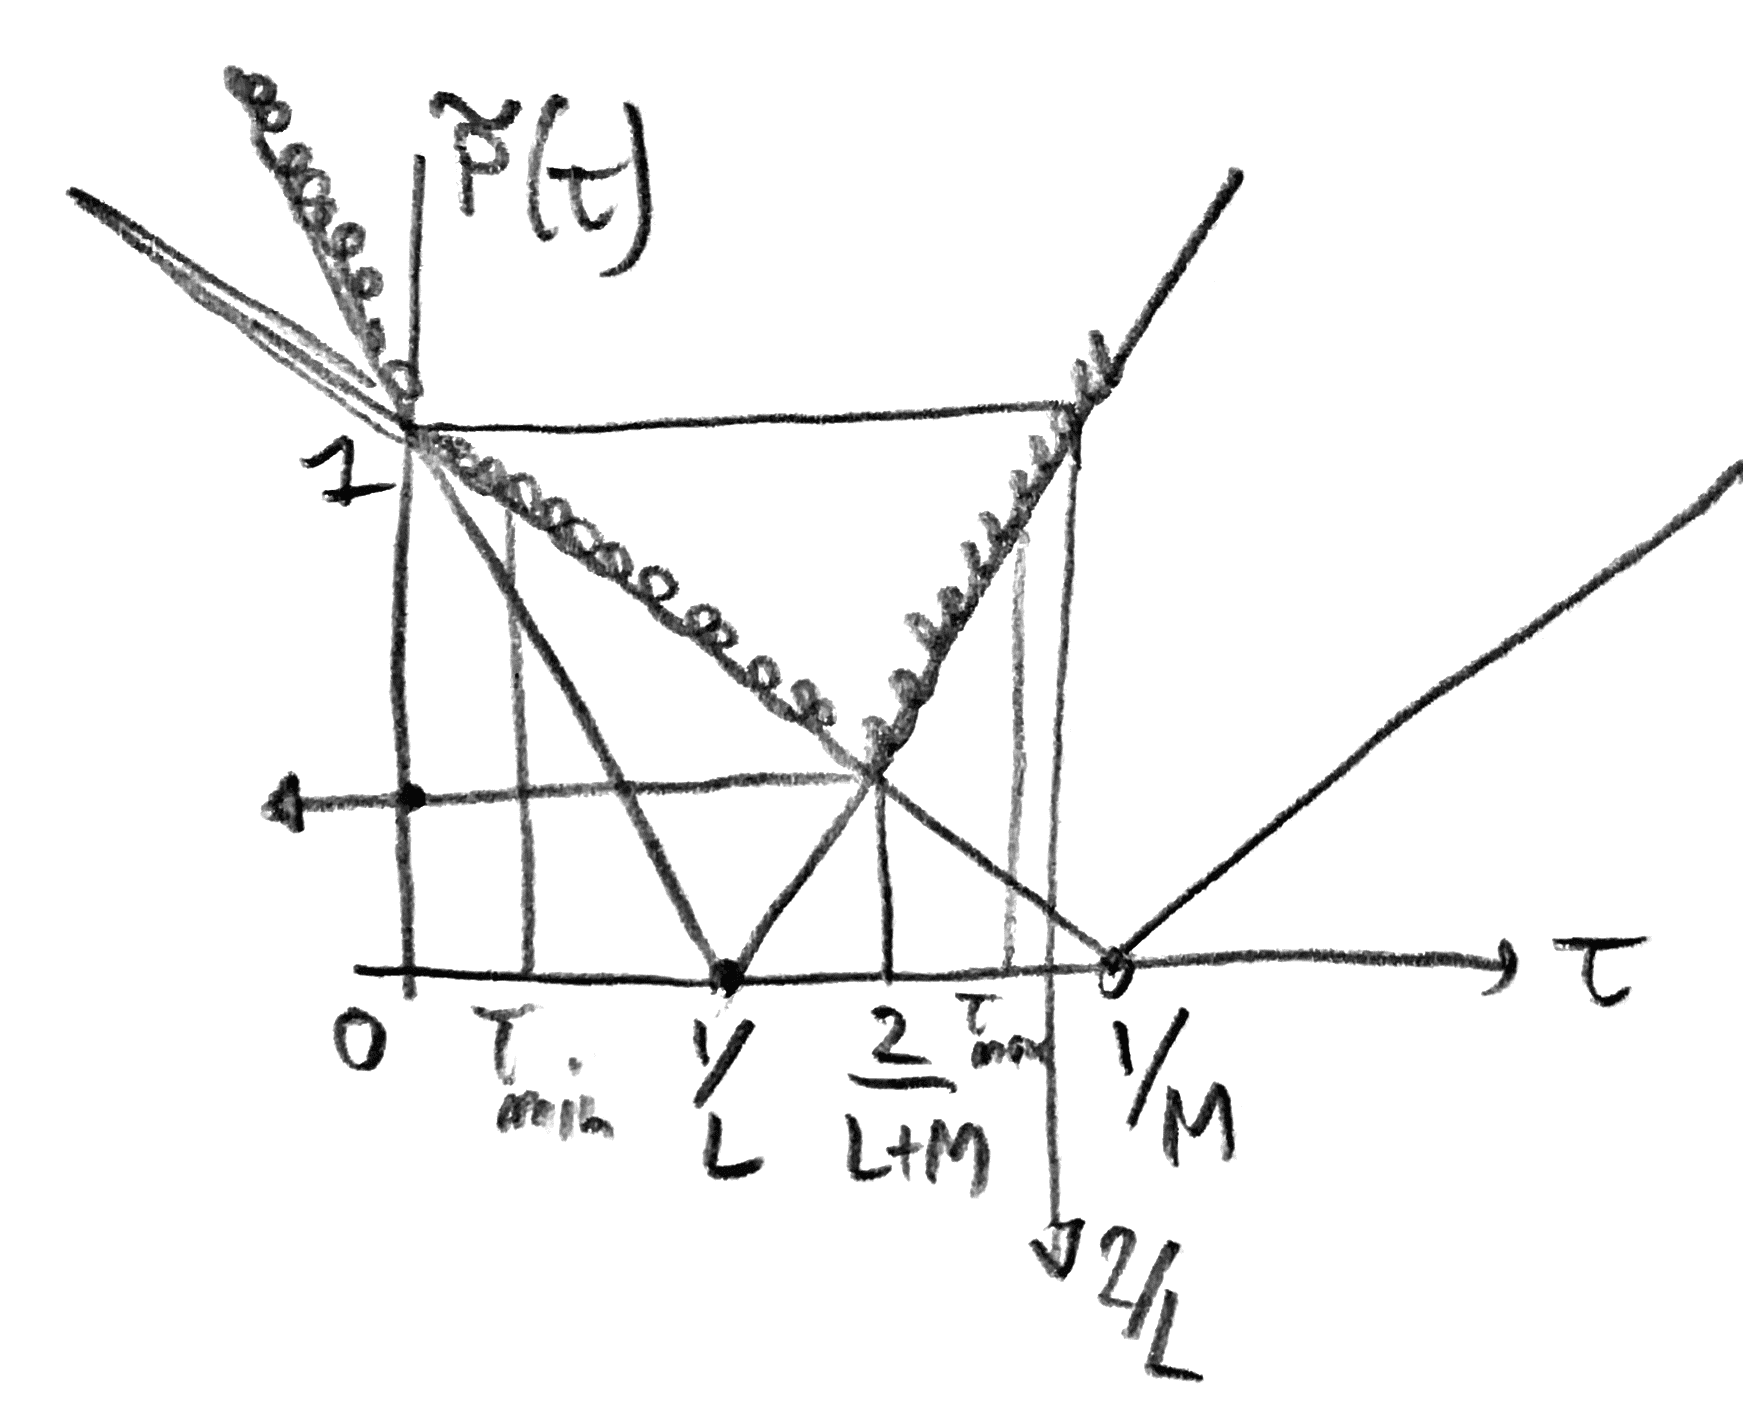
\includegraphics[width=.35\linewidth]{inverse-problems/grad-desc-linear}
\caption{\label{fig-grad-desc-contract}
Contraction constant $P(\tau)$ and $\tilde P(\tau)$ for a gradient descent step in the generic case (left) and for a quadratic function (right). 
}
\end{figure}

The error decay rate~\eqref{eq-global-linrate-grad}, although it is geometrical $O(\rho^\ell)$ is called a ``linear rate'' in the optimization literature. It is a ``global'' rate because it hold for all $\ell$ (and not only for large enough $\ell$).
%
The best (smallest) rate $\rho$ is obtained when choosing 
\eql{\label{eq-best-rate-global}
	\tau_\ell = \frac{\mu}{L^2}
	\qarrq
	\rho = 1 - \frac{\mu^2}{L^2}.
} 

In the case of a quadratic functional of the form~\eqref{eq-quad-func}, one can sharpen the convergence proof because the iterates are computed in closed form using matrix multiplication
\eq{
	\it{x}-x^\star = ( \Id_{N} - \tau_\ell A ) (\itz{x}-x^\star)
}
which leads to the following proposition (see also Figure~\ref{fig-grad-desc-contract}, right, for the corresponding contraction constant involved as a function of $\tau$).

\begin{prop}\label{prop-graddesc-quad}
	For $f(x)=\dotp{A}{f}-\dotp{b}{x}$ with the singular values of $A$ upper-bounded by $L$, assuming there exists $(\tau_{\min},\tau_{\max})$ such that
	\eql{\label{eq-descent-step-cond}
		0 < \tau_{\min} \leq \tau_\ell \leq \tilde\tau_{\max} < \frac{2}{L}
	}
	then there exists $0 \leq \tilde\rho<1$ such that 
	\eql{\label{eq-global-linrate-grad}
		\norm{ \it{x}-x^\star } \leq \tilde\rho^\ell \norm{\itz{x}-x^\star}.
	} 
	If the singular values are lower bounded by $\mu$, then the best rate $\tilde\rho$ is obtained for 
	\eql{\label{eq-best-rate-local}
		\tau_\ell = \frac{2}{L+\mu}
		\qarrq
		\tilde\rho \eqdef \frac{L-\mu}{L+\mu}.
	} 
\end{prop}


The maximum allowable step size $\tilde\tau_{\max}$ in~\eqref{eq-descent-step-cond} is much larger than $\tau_{\max}$ given in~\eqref{eq-descent-step-cond}, and the optimal rate~\eqref{eq-best-rate-local} is also much better (smaller) than the one in~\eqref{eq-best-rate-global}. In particular, if 
\eq{
	\epsilon \eqdef M/L \ll 1
} 
(which is the typical setup for ill-posed problems), then 
\eq{
	\rho \sim 1-\epsilon^2
	\qandq
	\tilde\rho \sim 1 - 2\epsilon.
}
The quantity $\epsilon$ in some sense reflects the inverse-conditioning of the problem. For quadratic function, it indeed corresponds exactly to the inverse of the condition number (which is the ratio of the largest to smallest singular value). The condition number is minimum and equal to $1$ for orthogonal matrices.

These two results are however complementary. Indeed, if the gradient descent converges, then ultimately $\it{x}$ is close to $x^\star$, so that one can approximate up to second order $f(x) \approx f(x^\star) + \dotp{Af}{f}-\dotp{f}{b}$ with $A=\partial^2 f(x^\star)$ and $b=-\nabla f(x^\star)$. So that the ``local'' rate, the one obtained after a large enough of iterations, is actually driven by $\tilde\rho$ and not $\rho$. It is thus important to distinguish between the global rate and the local rate. In practice, descent algorithm typically have two phase: a first ``slow'' phase govern by the global rate, and a second ``fast'' phase governed by the local rate. Unfortunately, the optimal step sizes $\tau_\ell$ are in general different for the two phase, so that optimal adaptation of step size is a difficult problems. This is why more advanced users typically use various line search strategies (to find the optimal step size at each iteration) or use second order information using quasi-Newton technics (BFGS).

The convergence result of Proposition~\ref{prop-graddesc-quad} does not requires strong convexity, while Theorem~\ref{thm-gradsec-strong-conv} does. In the general non-strongly convex case, it is still possible to prove convergence, but the rate is only sub-linear, and is only on the value of $f$, not on the iterate $\it{x}$ themselves.
%
Note that in this case, the solution of the minimization problem is not necessarily unique.
%
The proof is more technical.

\begin{thm}\label{thm-gradsec-non-strong-conv}
	If $f$ satisfy conditions~\eqref{eq-lipsch-grad}, assuming there exists $(\tau_{\min},\tau_{\max})$ such that
	\eql{\label{eq-descent-step-cond}
		0 < \tau_{\min} \leq \tau_\ell \leq \tau_{\max} < \frac{2}{L}, 
	}
	then $\it{x}$ converges to a solution $x^\star$ of~\eqref{eq-min-smooth-uncons} and
	there exists $C>0$ such that 
	\eql{\label{eq-sublin-rate-gd}
		f(\it{x})-f(x^\star) \leq \frac{C}{\ell+1}.
	} 
\end{thm}
\begin{proof}
	We only prove~\eqref{eq-sublin-rate-gd} since the proof that $\it{x}$ converges is more technical. Note indeed that if the minimizer $x^\star$ is non-unique, then it might be the case that the iterate $\it{x}$ ``cycle'' while approaching the set of minimizer, but actually convexity of $f$ prevents this kind of pathological behavior. 
	%
	For simplicity, we do the proof in the case $\tau_\ell = 1/L$, but it extends to the general case. 
	%
	The $L$-smoothness property imply~\eqref{eq-above-below-quad}, which reads
	\eq{
	f(\iit{x}) 
		\leq 
		f(\it{x}) + \dotp{\nabla f(\it{x})}{\iit{x}-\it{x}} + \frac{L}{2}\norm{\iit{x}-\it{x}}^2.
	}
	Using the fact that $\iit{x}-\it{x} = -\frac{2}{L} \nabla f(\it{x})$, one obtains
	\eql{\label{eq-proox-x'rad-nonstrong-1}
		f(\iit{x}) 
		\leq 
		f(\it{x}) -  \norm{\nabla f(\it{x})}^2
		\leq 
		f(\it{x}) - \frac{1}{2L} \norm{\nabla f(\it{x})}^2
	}
	This shows that $(f(\it{x}))_\ell$ is a decaying sequence.
	%
	By convexity
	\eq{
		f(\it{x}) + \dotp{\nabla f(\it{x})}{x^\star-\it{x}}�\leq  f(x^\star)
	}
	and plugging this in~\eqref{eq-proox-x'rad-nonstrong-1} shows
	\begin{align*}
		f(\iit{x})  &\leq   
		f(x^\star) - \dotp{\nabla f(\it{x})}{x^\star-\it{x}} - \frac{1}{2L} \norm{\nabla f(\it{x})}^2 \\
		&= f(x^\star) + \frac{L}{2}\pa{
			\norm{\it{x}-x^\star}^2 - \norm{\it{x}-x^\star-\frac{1}{L}\nabla f(\it{x})}^2
		}\\
		&= f(x^\star) + \frac{L}{2}\pa{
			\norm{\it{x}-x^\star}^2 - \norm{x^\star-\iit{x}}^2 }.
	\end{align*}
	Summing these inequalities for $\ell=0,\ldots,k$, one obtains
	\eq{
		\sum_{\ell=1}^k f(\iit{x}) - k x^\star \leq  \frac{L}{2}\pa{
			\norm{\itz{x}-x^\star}^2 - \norm{x^{(k+1)}-x^\star}^2 }
	}
	and since $f(\iit{x})$ is decaying $\sum_{\ell=1}^k f(\iit{x}) \geq (k+1) f(x^{(k+1)})$, thus 
	\eq{
		f(x^{(k+1)}) - f(x^\star) \leq \frac{L \norm{\itz{x}-x^\star}^2}{2(k+1)}
	}
	which gives~\eqref{eq-sublin-rate-gd} for $C \eqdef L \norm{\itz{x}-x^\star}^2/2$.
\end{proof}


%%%%%%%%%%%%%%%%%%%%%%%%%%%%%%%%%%%%%%%%%%%%%%%%
\subsection{Sub-gradient Descent}

The gradient descent~\eqref{eq-grad-desc} cannot be applied on a non-smooth function $f$. One can use in place of a gradient a sub-gradient, which defines the sub-gradient descent
\eql{\label{eq-subgrad-desc}
	\iit{x} \eqdef \it{x} - \tau_\ell \it{g}
	\qwhereq
	\it{g} \in \partial f( \it{x} ).
}
The main issue with this scheme is that to ensure convergence, the iterate should go to zero. One can easily convince oneself why by looking at the iterates on a function $f(x)=|x|$.

\begin{thm}
	If $\sum_{\ell} \tau_\ell=+\infty$ and $\sum_{\ell} \tau_\ell^2 < +\infty$, then $\it{x}$ converges to a minimizer of $f$. 
\end{thm}

%%%%%%%%%%%%%%%%%%%%%%%%%%%%%%%%%%%%%%%%%%%%%%%%%%%%%%%%%%%%%%%%%%%%%%%%%%%%%%%%%%
\subsection{Projected Gradient Descent}
\label{sec-proj-grad}

We consider a generic constraint optimization problem as
\eql{\label{eq-constr}
	\umin{x \in \Cc} f(x) 
} 
where $\Cc \subset \RR^S$ is a closed convex set and $f : \RR^S \rightarrow \RR$ is a smooth convex function (at least of class $\Cc^1$). 

The gradient descent algorithm~\eqref{eq-grad-desc}�is generalized to solve a constrained problem using the projected gradient descent 
\eql{\label{eq-proj-grad-desc}
	\iit{x} \eqdef \Proj_\Cc \pa{ \it{x} - \tau_\ell \nabla f( \it{x} ) }, 
}
where $\Proj_\Cc$ is the orthogonal projector on $\Cc$
\eq{
	\Proj_\Cc(x) = \uargmin{x' \in \Cc} \norm{x-x'}
}
which is always uniquely defined because $\Cc$ is closed and convex.
%
The following proposition shows that all the convergence properties of the classical gradient descent caries over to this projected algorithm.

\begin{thm}\label{thm-proj-grad}
	Theorems~\ref{thm-gradsec-strong-conv} and~\ref{thm-gradsec-non-strong-conv} still holds when replacing iterations~\eqref{eq-grad-desc} by~\eqref{eq-proj-grad-desc}.
\end{thm}

\begin{proof}
	The proof of Theorem~\ref{thm-gradsec-strong-conv} extends because the projector is contractant, 
	$\norm{\Proj_\Cc(x)-\Proj_\Cc(x')} \leq \norm{x-x'}$ so that the strict contraction properties of the gradient descent is maintained by this projection.   
\end{proof}

The main bottleneck that often prevents to use~\eqref{eq-proj-grad-desc} is that the projector is often complicated to compute. We are however lucky since for $\ell^1$ mininization, one can apply in a straightforward manner this method. 





%%%%%%%%%%%%%%%%%%%%%%%%%%%%%%%%%%%%%%%%%%%%%%%%%%%%%%%%%%%%%%%%%%%%%%%%%%%%%%%%%%
%%%%%%%%%%%%%%%%%%%%%%%%%%%%%%%%%%%%%%%%%%%%%%%%%%%%%%%%%%%%%%%%%%%%%%%%%%%%%%%%%%
%%%%%%%%%%%%%%%%%%%%%%%%%%%%%%%%%%%%%%%%%%%%%%%%%%%%%%%%%%%%%%%%%%%%%%%%%%%%%%%%%%
\section{Proximal Operators}

For non-smooth functions $f$, it is not possible to perform an ``explicit'' gradient descent step because the gradient is not even defined. One thus needs to replace this ``explicit''  step by an ``implicit'' one, which is possible even if $f$ is non-smooth.


%%%%%%%%%%%%%%%%%%%%%%%%%%%%%%%%%%%%%%%%%%%%%%%%
\subsection{Proximal Map }

The implicit stepping of amplitude $\tau>0$ is defined as 
\eql{\label{eq-defn-proximal}
	\foralls x, \quad
	\Prox_{\tau f}(x) \eqdef \uargmin{x'} \frac{1}{2}\norm{x-x'}^2 + f(x').
}
It amounts to minimize function $f$ locally around $x$, in a ball of radius controlled by $\tau$.
%
This the involved function $\frac{1}{2}\norm{x-\cdot}^2 + f$ is strongly convex, this operator $\Prox_{\tau f}$ is well defined and single-valued. 

When $f=\iota_\Cc$ is an indicator, the proximal map boils down to a projection $\Prox_{\iota_\Cc}=\Proj_{\Cc}$, it is thus in some sense a generalization of the projection to arbitrary function. And can also be interpreted as a projector on a level set of $f$. 

%%%
\paragraph{Examples}


As  simple examples, let us list
\eq{
	\Prox_{\frac{\tau}{2} \norm{\cdot}^2}(x) =  \frac{x}{1+\tau}, 
	\qandq
	\Prox_{\tau \norm{\cdot}_1} = \Ss_\tau^1(x), 
}
where the soft-thresholding is defined as
\eq{
	\Ss_\tau^1(x) = ( S_\tau(x_i) )_{i=1}^N \qwhereq
	S_\tau(r) = \sign(r) (|r|-\la)_+, 
}
(see also~\eqref{eq-soft-thresh}).

Note that in some case, the proximal map of a non-convex function is well defined, for instance
$\Prox_{\tau \norm{\cdot}_0}$ is the hard thresholding associated to the threshold $\sqrt{2\tau}$, see Proposition~\ref{prop-equiv-sparse-thresh}.


%%%
\paragraph{Basic properties.}

If $f(x)=\sum_{k=1}^K f(x_k)$ for $x=(x_1,\ldots,x_K)$ is separable, then
\eq{
	\Prox_{\tau f}(x) = ( \Prox_{\tau f_k}(x_k) )_{k=1}^K.
}
The following proposition is very useful.

\begin{prop}
	If $A \in \RR^{P \times N}$ is a tight frame, i.e. $AA^*=\Id_P$, then 
	\eq{
		\Prox_{f \circ A} = A^* \circ \Prox_{f} \circ A + \Id_N - A^* A.
	}
	In particular, if $A$ is orthogonal, then $\Prox_{f \circ A} = A^* \circ \Prox_{f} \circ A$.
\end{prop}

%%%
\paragraph{Link with sub-differential.}

For a set-valued map $U : \Hh \hookrightarrow \Gg$, we define the inverse set-valued map $U^{-1} : \Gg \hookrightarrow \Hh$ by 
\eq{
	h \in U^{-1}(g) 
	\quad\Longleftrightarrow\quad
	g \in U(h) 
} 

% TODO: add picture

One has the following equivalence
\eq{
	z = \Prox_{\tau f}(x) 
	\Leftrightarrow
	0 \in z-x+\tau\partial f(z)
	\Leftrightarrow
	x \in (\Id+\tau\partial f)(z)
	\Leftrightarrow
	z = (\Id+\tau\partial f)^{-1}(x)
}	
where for the last equivalence, we have replace ``$\in$'' by ``$=$'' because the proximal map is single valued.
%
The proximal operator is hence often referred to the ``resolvent'' $\Prox_{\tau f} = (\Id+\tau\partial f)^{-1}$ of the maximal monotone operator $\partial f$. 
% 


%%%%%%%%%%%%%%%%%%%%%%%%%%%%%%%%%%%%%%%%%%%%%%%%
\subsection{Proximal Point Algorithm}

One has the following equivalence 
\begin{align}\label{eq-proxpoint-fix}
	x^\star \in \argmin f
	&\quad\Leftrightarrow\quad
	0 \in \partial f(x^\star)
	\quad\Leftrightarrow\quad
	x^\star \in (\Id+\tau \partial f)(x^\star) \\
	&\quad\Leftrightarrow\quad
	x^\star = (\Id+\tau \partial f)^{-1}(x^\star) = \Prox_{\tau f}(x^\star).
\end{align}
This shows that being a minimizer of $f$ is equivalent to being a fixed point of $\Prox_{\tau f}$.
%
This suggest the following fixed point iterations, which are called the proximal point algorithm 
\eql{\label{eq-proximal-point}
	\iit{x} \eqdef \Prox_{\tau_\ell f}(\it{x}).
}
On contrast to the gradient descent fixed point scheme, the proximal point method is converging for any sequence of steps.

\begin{thm}
	If $0<\tau_{\min} \leq \tau_\ell \leq \ga_{\max} < +\infty$, then $\it{x} \rightarrow x^\star$ a minimizer of $f$.
\end{thm}

This implicit step~\eqref{eq-proximal-point} should be compared with a gradient descent step~\eqref{eq-grad-desc}
\eq{
	\iit{x} \eqdef (\Id+\tau_\ell \nabla f)(\it{x}).
}
One sees that the implicit resolvent $(\Id-\tau_\ell \partial f)^{-1}$ replaces the explicit step $\Id+\tau_\ell \nabla f$. For small $\tau_\ell$ and smooth $f$, they are equivalent at first order. But the implicit step is well defined even for non-smooth function, and the scheme (the proximal point) is always convergent (whereas the explicit step size should be small enough for the gradient descent to converge). This is inline with the general idea the implicit stepping (e.g. implicit Euler for integrating ODE, which is very similar to the proximal point method) is more stable. Of course, the drawback is that explicit step are very easy to implement whereas in general proximal map are hard to solve (most of the time as hard as solving the initial problem).


%%%%%%%%%%%%%%%%%%%%%%%%%%%%%%%%%%%%%%%%%%%%%%%%
\subsection{Forward-Backward}
\label{sec-fb}

It is in general impossible to compute $\Prox_{\ga f}$ so that the proximal point algorithm is not implementable.
%
In oder to derive more practical algorithms, it is important to restrict the class of considered function, by imposing some structure on $f$. We consider functions of the form
\eql{\label{eq-fb-split}
	f(x) =  \Ff(x) +  \Gg(x)
}
where $\Gg \in \Ga_0(\Hh)$ can be an arbitrary, but $\Ff$ needs to be smooth.

One can modify the fixe point derivation~\eqref{eq-proxpoint-fix} to account for this special structure
\begin{align*}
 	x^\star \in \argmin \Ff + \Gg
	& \quad\Leftrightarrow\quad
	0 \in \nabla \Ff(x^\star) + \partial \Gg(x^\star) 
	\quad\Leftrightarrow\quad
	x^\star - \tau \nabla \Ff(x^\star) \in (\Id+\tau \partial \Gg)(x^\star) \\
	& \quad\Leftrightarrow\quad
	x^\star = ( \Id + \tau \partial \Gg )^{-1} \circ ( \Id - \tau \nabla \Ff ) (x^\star).
\end{align*}
This fixed point suggests the following algorithm, with the celebrated Forward-Backward
\eql{\label{eq-fb}
		\iit{x} \eqdef \Prox_{\tau_\ell \Gg}\pa{ \it{x} - \tau_\ell \nabla\Ff(\it{x}) }.
}


%%%
\paragraph{Derivation using surrogate functionals.}

An intuitive way to derive this algorithm, and also a way to prove its convergence, it using the concept of surrogate functional.

%
% The difficulty is the presence of the operator $A$ in the $\ldeux$ norm, which makes this problem significantly more difficult than the simple denoising by regularization\eqref{eq-regul-denoising}.

To derive an iterative algorithm, we modify the energy $f(x)$ to obtain a surrogate functional $f(x,\it{x})$ whose minimization corresponds to a simpler optimization problem, and define the iterations as
\eql{\label{eq-surrogate-iter}
	\iit{x} \eqdef \uargmin{x} f(x,\it{x}).
}
In order to ensure convergence, this function should satisfy the following property
\eql{\label{eq-surrogate-pty}
	f(x) \leq f(x,x')
	\qandq
	f(x,x) = f(x)
}
and $f(x)-f(x,x')$ should be a smooth function.
%
Property \eqref{eq-surrogate-pty} guarantees that $f$ is decaying by the iterations
\eq{
	f(\iit{x}) \leq f(\it{x})
}
and it simple to check that actually all accumulation points of $(\it{x})_\ell$ are stationary points of $f$. 

In order to derive a valid surrogate $f(x,x')$ for our functional~\eqref{eq-fb-split}, since we assume $\Ff$ is $L$-smooth (i.e. satisfies~\eqref{eq-lipsch-grad}), let us recall the quadratic majorant~\eqref{eq-above-below-quad}
\eq{
	\Ff(x) 
	\leq 
	\Ff(x') + \dotp{\nabla \Ff(x')}{x'-x} + \frac{L}{2}\norm{x-x'}^2, 
}
so that for $0 < \tau < \frac{1}{L}$, the function 
\eql{\label{eq-surrogate-ip}
	f(x,x') \eqdef \Ff(x') + \dotp{\nabla \Ff(x')}{x'-x} + \frac{1}{2\tau}\norm{x-x'}^2 + \Gg(x)
}
satisfies the surrogate conditions~\eqref{eq-surrogate-pty}.
%
The following proposition shows that minimizing the surrogate functional corresponds to the computation of a so-called proximal operator. 

\begin{prop}
	The update~\eqref{eq-surrogate-iter} for the surrogate~\eqref{eq-surrogate-ip} is exactly~\eqref{eq-fb}.
\end{prop}
\begin{proof}
	This follows from the fact that
	\eq{
		\dotp{\nabla \Ff(x')}{x'-x} + \frac{1}{2\tau}\norm{x-x'}^2 
		= \frac{1}{2\tau} \norm{ x - (x'-\tau \nabla\Ff(x'))  }^2 + \text{cst}.
	}
\end{proof}

%%%
\paragraph{Convergence of FB. }

Although we impose $\tau<1/L$ to ensure majorization property, one can actually show convergence under the same hypothesis as for the gradient descent, i.e. $0 < \tau < 2/L$, with the same convergence rates.  This means that Theorem~\ref{thm-proj-grad} for the projected gradient descent extend to FB. 

\begin{thm}\label{thm-fb-conv}
	Theorems~\ref{thm-gradsec-strong-conv} and~\ref{thm-gradsec-non-strong-conv} still holds when replacing iterations~\eqref{eq-grad-desc} by~\eqref{eq-fb}.
\end{thm}

Note furthermore that the projected gradient descent algorithm~\eqref{eq-proj-grad-desc} is recovered as a special case of~\eqref{eq-fb} when setting $J=\iota_{\Cc}$ the indicator of the constraint set, since $\Prox_{\rho J} = \Proj_{\Cc}$ in this case.

Of course the difficult point is to be able to compute in closed form $\Prox_{\tau \Gg}$ in~\eqref{eq-fb}, and this is usually possible only for very simple function. We have already seen such an example in Section~\ref{sec-ista} for the resolution of $\ell^1$-regularized inverse problems (the Lasso).


%%%%%%%%%%%%%%%%%%%%%%%%%%%%%%%%%%%%%%%%%%%%%%%%%%%%%%%%%%%%%%%%%%%%%%%%%%%%%%%%%%
%%%%%%%%%%%%%%%%%%%%%%%%%%%%%%%%%%%%%%%%%%%%%%%%%%%%%%%%%%%%%%%%%%%%%%%%%%%%%%%%%%
%%%%%%%%%%%%%%%%%%%%%%%%%%%%%%%%%%%%%%%%%%%%%%%%%%%%%%%%%%%%%%%%%%%%%%%%%%%%%%%%%%
\section{Primal-Dual Algorithms}

%%%%%%%%%%%%%%%%%%%%%%%%%%%%%%%%%%%%%%%%%%%%%%%%
\subsection{Forward-backward on the Dual}
\label{sec-fb-dual}

\paragraph{Chambolle's algorithm.}

Chambolle in \cite{chambolle-algo-tv}�detail an algorithm to minimize exactly the TV denoising problem
\eql{\label{eq-prox-tv}
	x_\la^\star = \uargmin{x \in \Hh} \frac{1}{2} \norm{x-x'}^2 + \la \normTV{x}.
}
It uses a relationship between the vectorial $\lun$ and $\linf$ norms
\eq{
	\normu{v} = \sum_{m=0}^{N-1} \norm{v_m} \qandq
	\normi{v} = \umax{0 \leq m < N} \norm{v_m}
}
where each $v_m \in \RR^2$ and $v \in \RR^{N \times 2}$. One has
\eq{
	\normu{v} = \umax{ \normi{w} \leq 1 } \dotp{w}{u}
}
which allows one to re-write the optimization \eqref{eq-prox-tv} as
\eq{
	\umin{x \in \Hh} \umax{\normi{w} \leq 1} 
		\frac{1}{2} \norm{x-x'}^2 + \la \dotp{w}{\nabla g}.
}
Exchanging the roles of the min and the max, one proves that the solution of  \eqref{eq-prox-tv} is re-written as
\eql{\label{eq-primal-dual-chambolle}
	x_\la^\star =  x + \la \diverg(w^\star)
}
where 
\eql{\label{eq-chambolle-dual}
	w^\star \in \uargmin{\normi{w} \leq 1} \norm{f + \la \diverg(w^\star)}^2.
}
The convex optimization problem \eqref{eq-chambolle-dual} computes a dual vector field $w^\star \in \RR^{N \times 2}$, from which the denoised image is recovered using \eqref{eq-primal-dual-chambolle}.

The dual problem \eqref{eq-chambolle-dual} is the minimization of a quadratic functional subject to a convex $\linf$ constraint. It can thus be solved using for instance a projected gradient descent
\eq{
	w^{(k+1)}_m = \frac{ \tilde w^{(k)}_m }{ \max(|\tilde w^{(k)}_m|,1) }
	\qwhereq
	\tilde w^{(k)} = w^{(k)} + \tau \nabla( f/\la + \diverg(w^{(k)}) ).
}  
If the gradient step size satisfy $0 < \tau < 1/4$, one can prove that 
\eq{
	f + \la \diverg(w^{(k)}) \longrightarrow f_\la^\star
	\qwhenq
	k \rightarrow +\infty.
}


%%%%%%%%%%%%%%%%%%%%%%%%%%%%%%%%%%%%%%%%%%%%%%%%
\subsection{Douglas-Rachford}


%%%%%%%%%%%%%%%%%%%%%%%%%%%%%%%%%%%%%%%%%%%%%%%%
\subsection{Primal-Dual Splitting}

